\subsubsection{Convergencia}

En este experimento buscamos estudiar la convergencia del método de la potencia. Para ello generamos dos instancias. La primera instancia fue generada con 2.500 vértices y 2.500 aristas. La segunda fue generada con 5000 vértices, utilizando las mismas aristas. Ambas instancias fueron generadas con un $\alpha = 0.85$. Como criterio de parada, se utilizo que la diferencia entre las normas 1 de dos vectores en sucesiones consecutivas sea menor a $\epsilon = 10^{-5}$. A continuación mostramos los resultados:

\begin{figure}[h]
  \centering
  \begin{minipage}[b]{0.49\textwidth}
  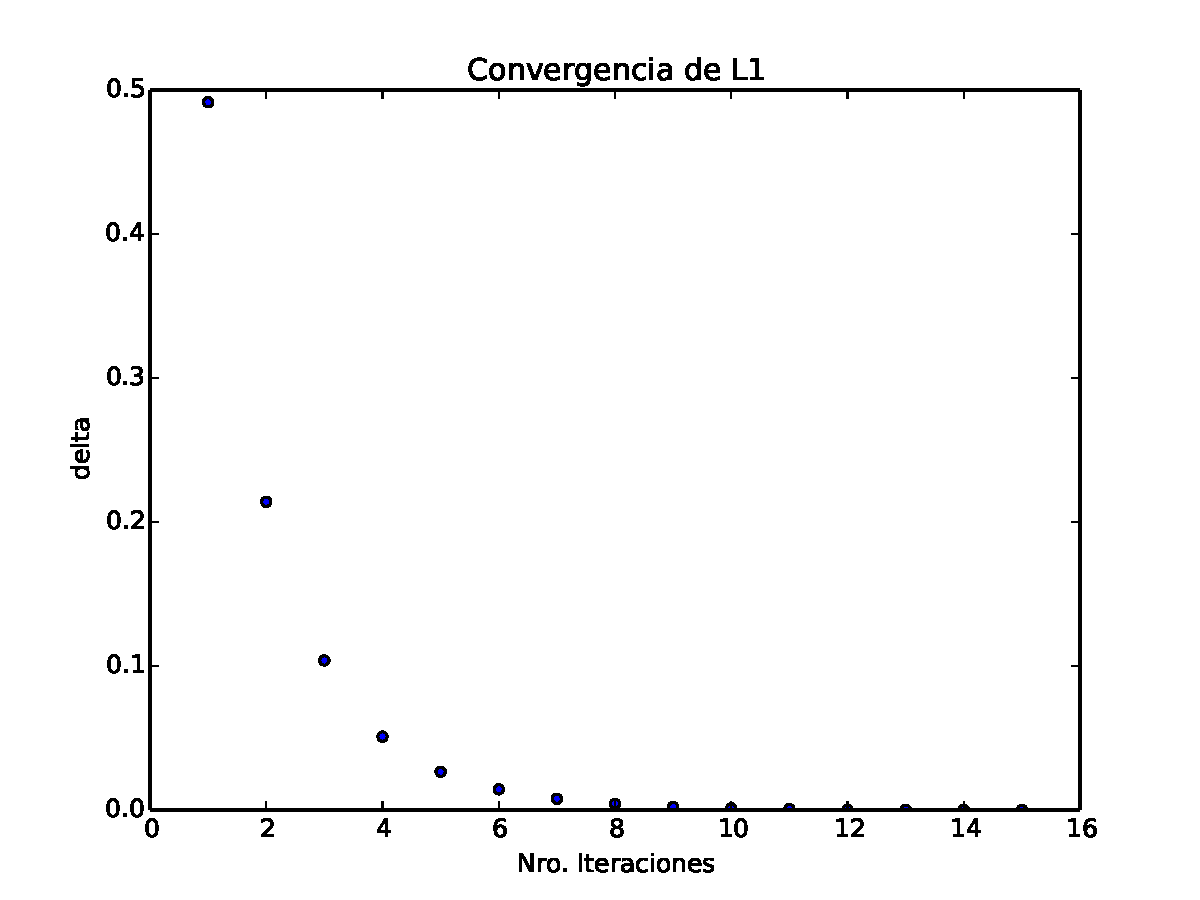
\includegraphics[scale=0.5]{images/conv_2265.pdf}
  \caption{2500 vértices}
  \end{minipage}
  \hfill
  \begin{minipage}[b]{0.49\textwidth}
  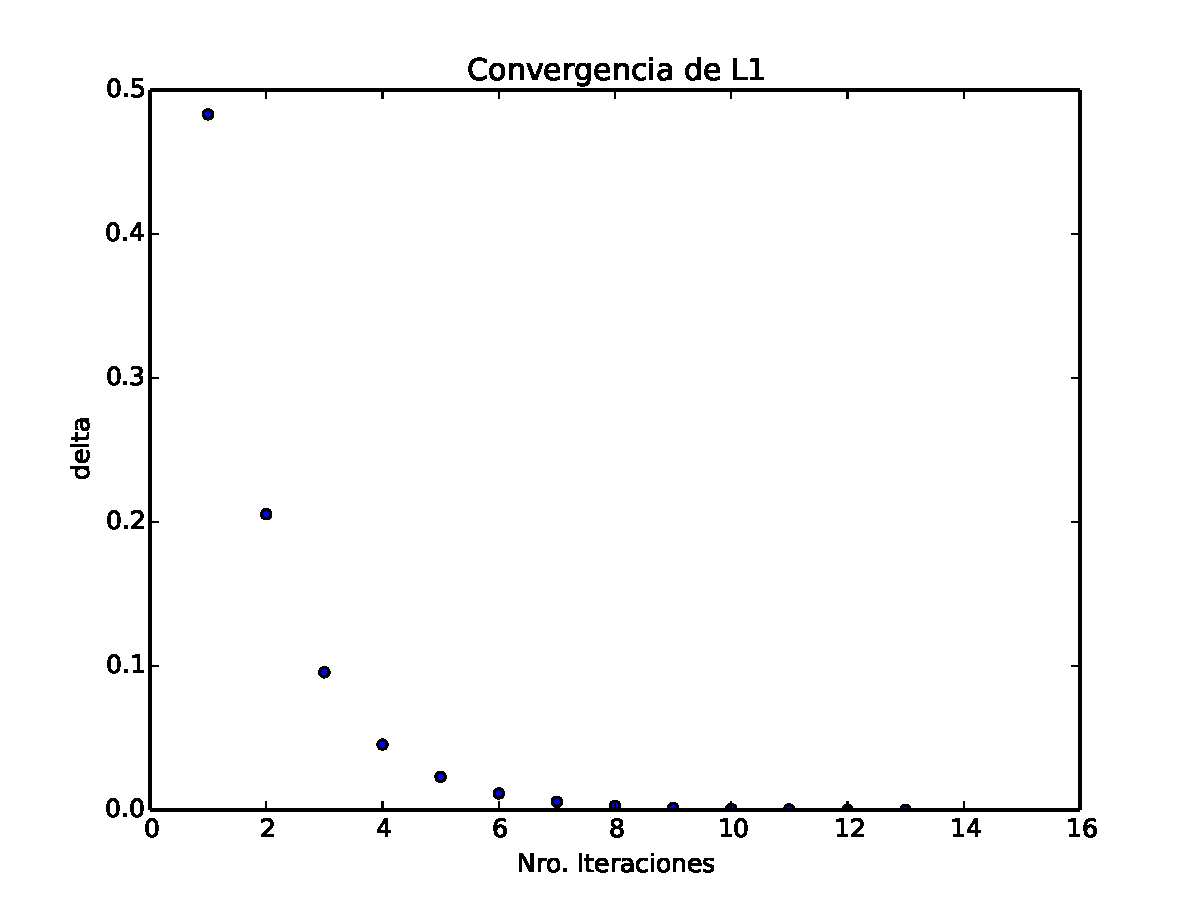
\includegraphics[scale=0.5]{images/conv_5000.pdf}
  \caption{5000 vértices}
  \end{minipage}
\end{figure}

Como podemos observar en ambos gráficos, a medida que aumenta el numero de iteraciones el delta baja de forma monótona. A su vez, en general ambos algoritmos toman aproximadamente 13 iteraciones en converger. Notar lo siguiente, que la cantidad de vértices se mayor no implica necesariamente que el método de la potencia tome mas iteraciones en converger. De hecho, podemos observar que la instancia con 5000 vértices toma 13 iteraciones, mientras que con 2500 vértices toma 15 iteraciones.